
\begin{figure}
	\begin{tabular}{cc}
		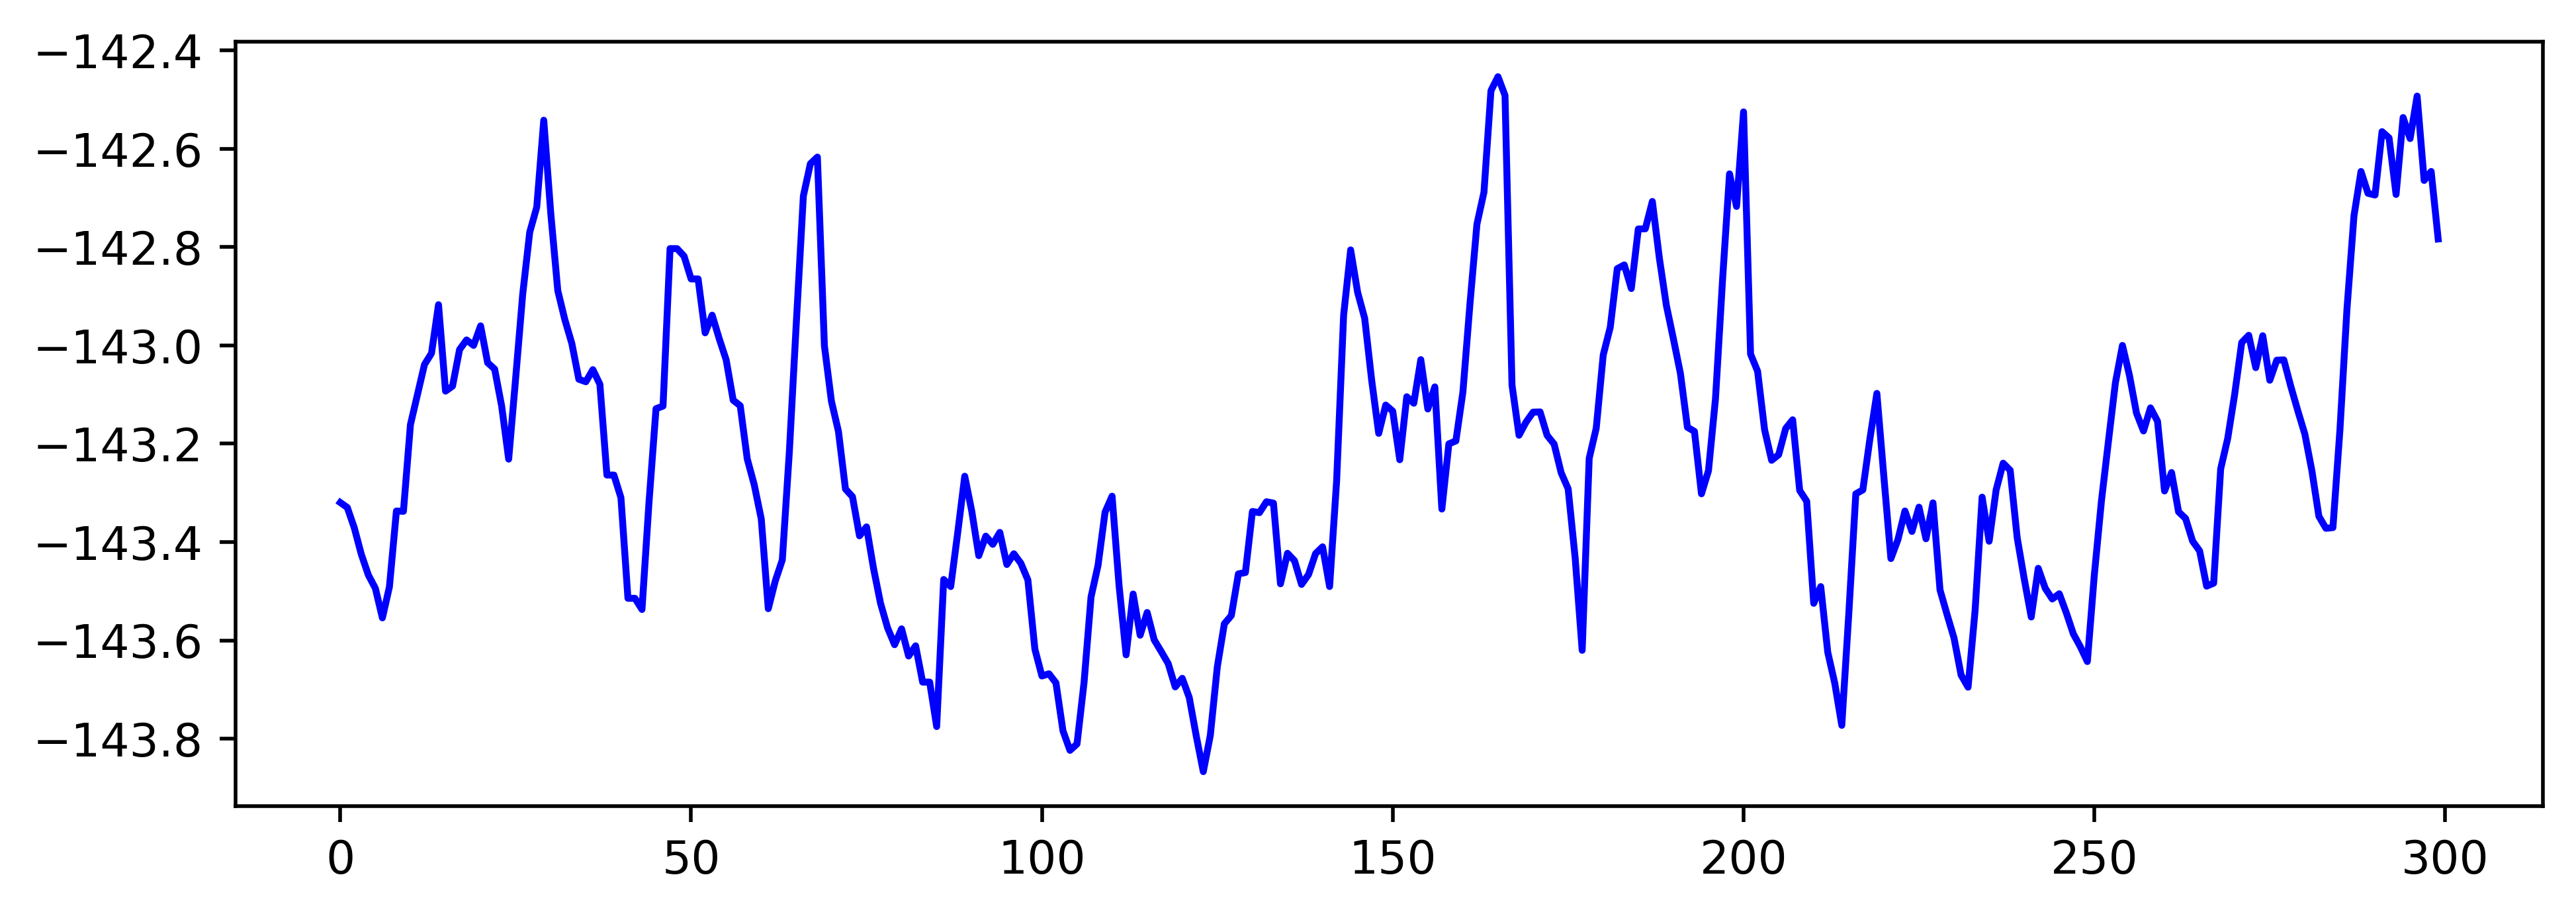
\includegraphics[width=0.45\linewidth]{img/samples/butppg_111001.png} 
			& 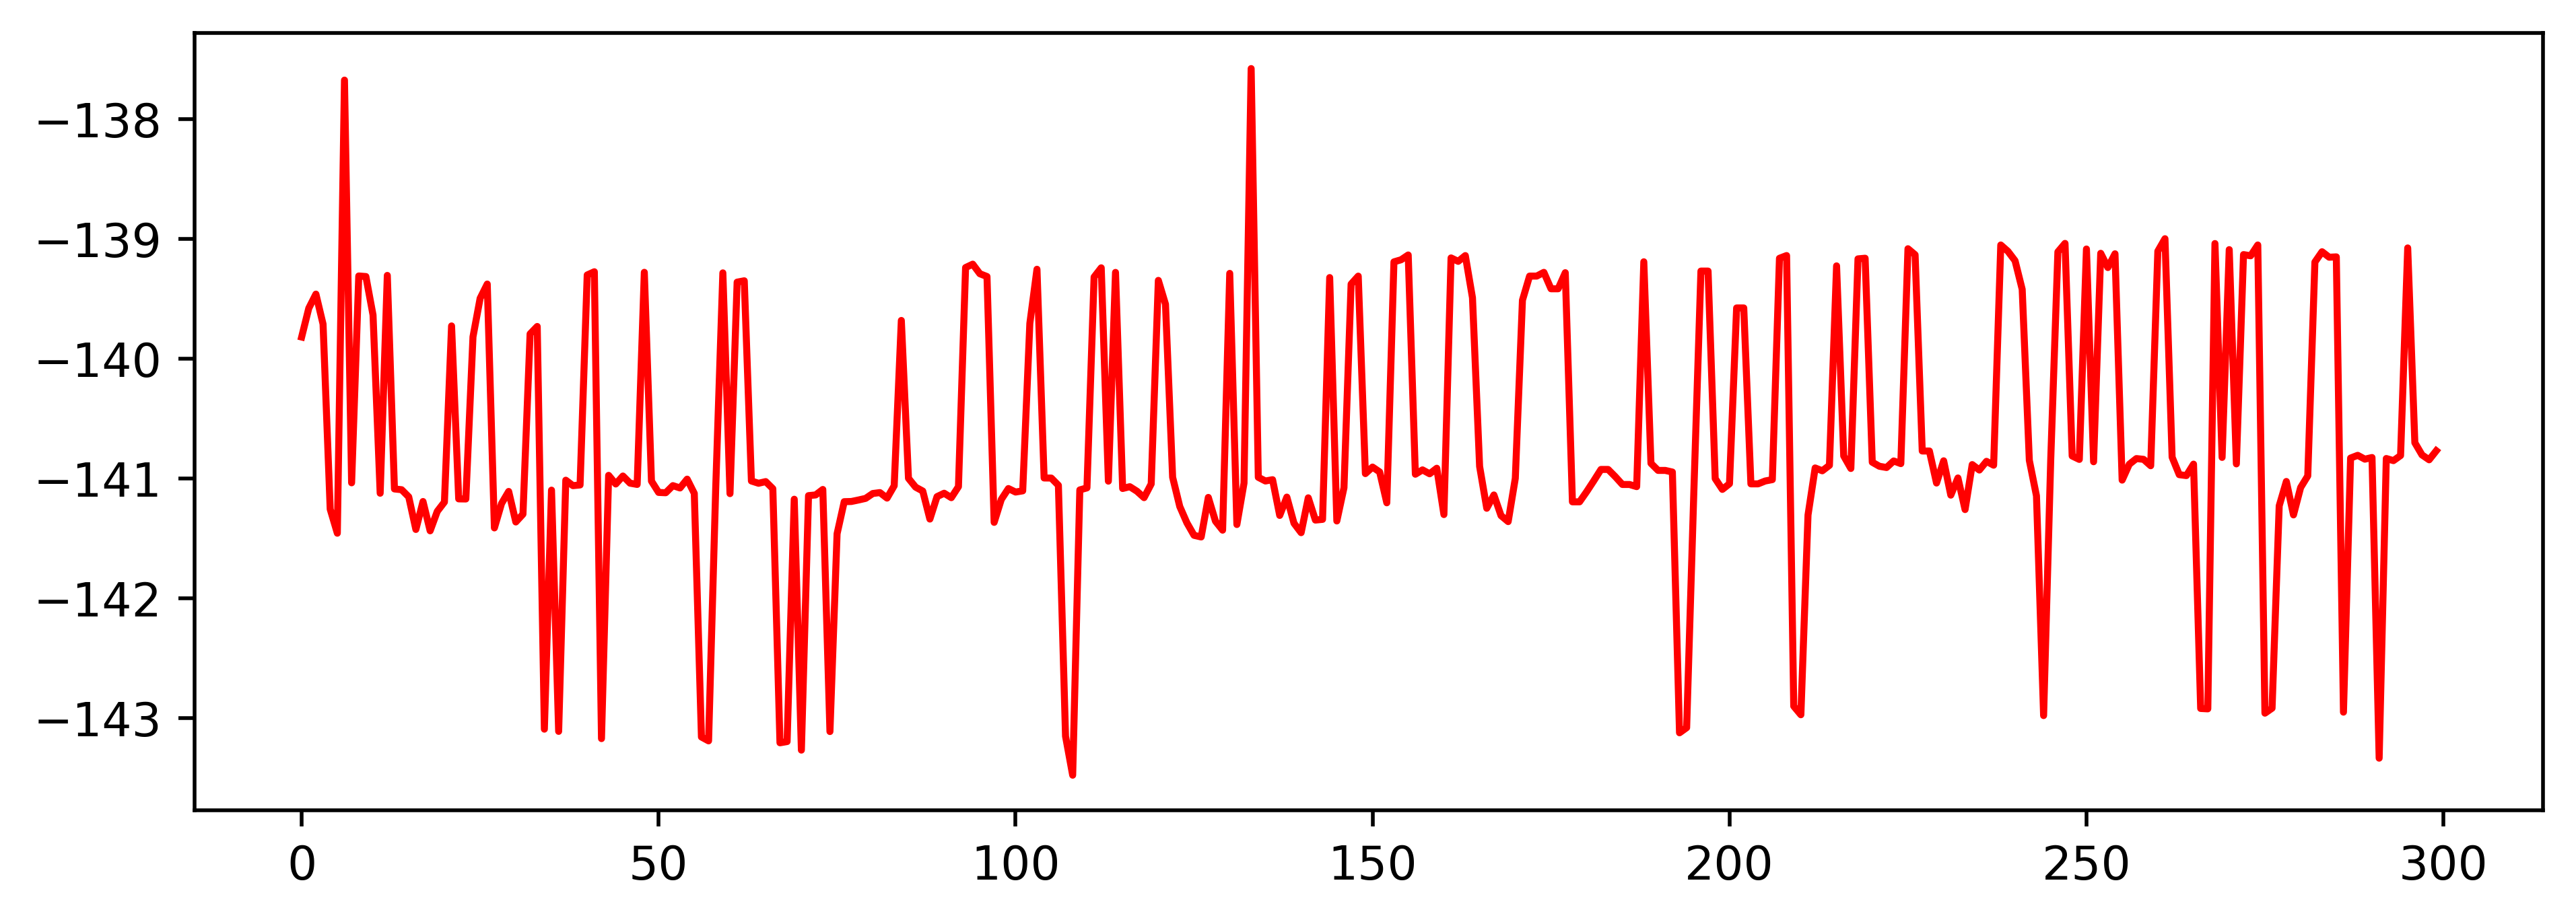
\includegraphics[width=0.45\linewidth]{img/samples/butppg_111003.png} \\
		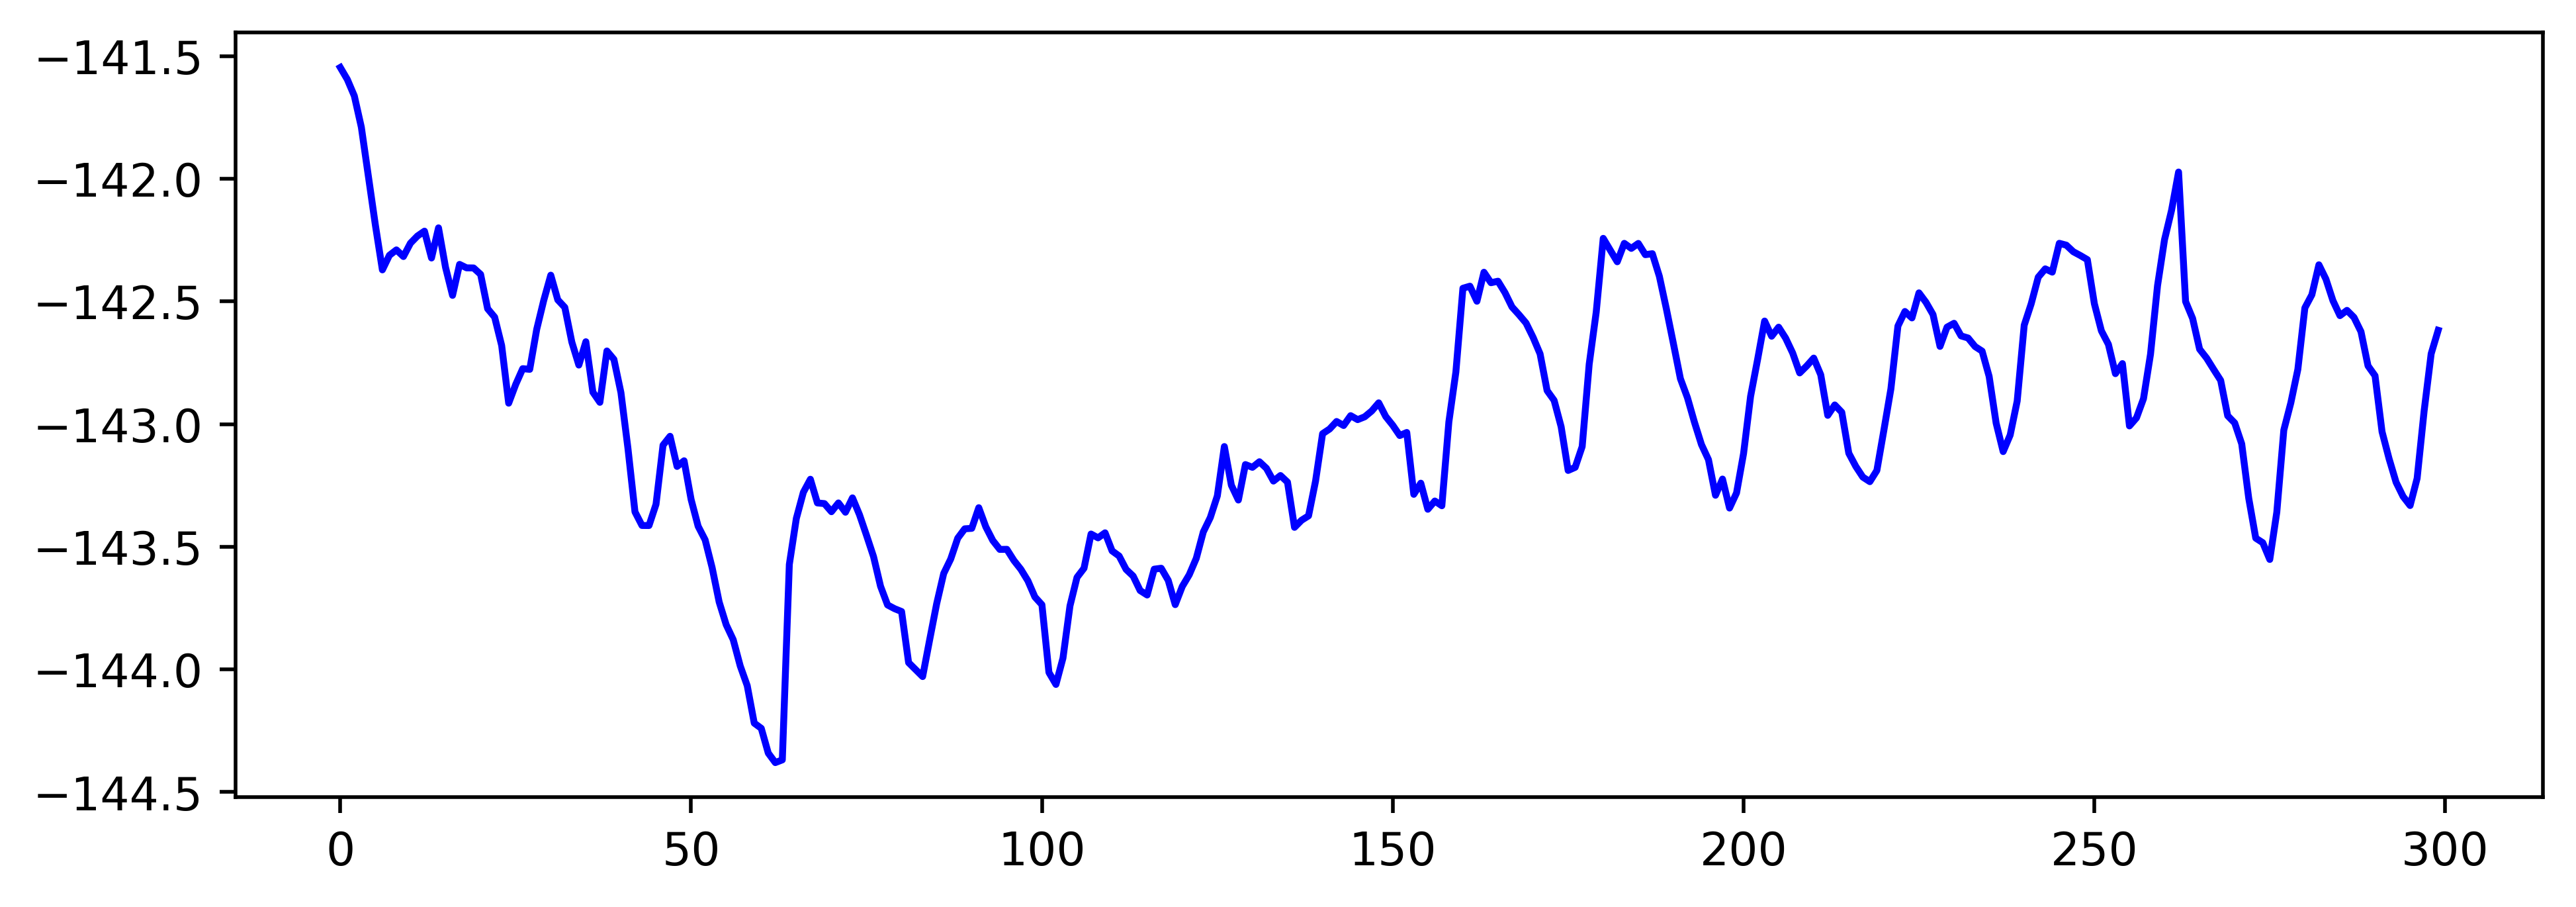
\includegraphics[width=0.45\linewidth]{img/samples/butppg_111002.png} 
			& 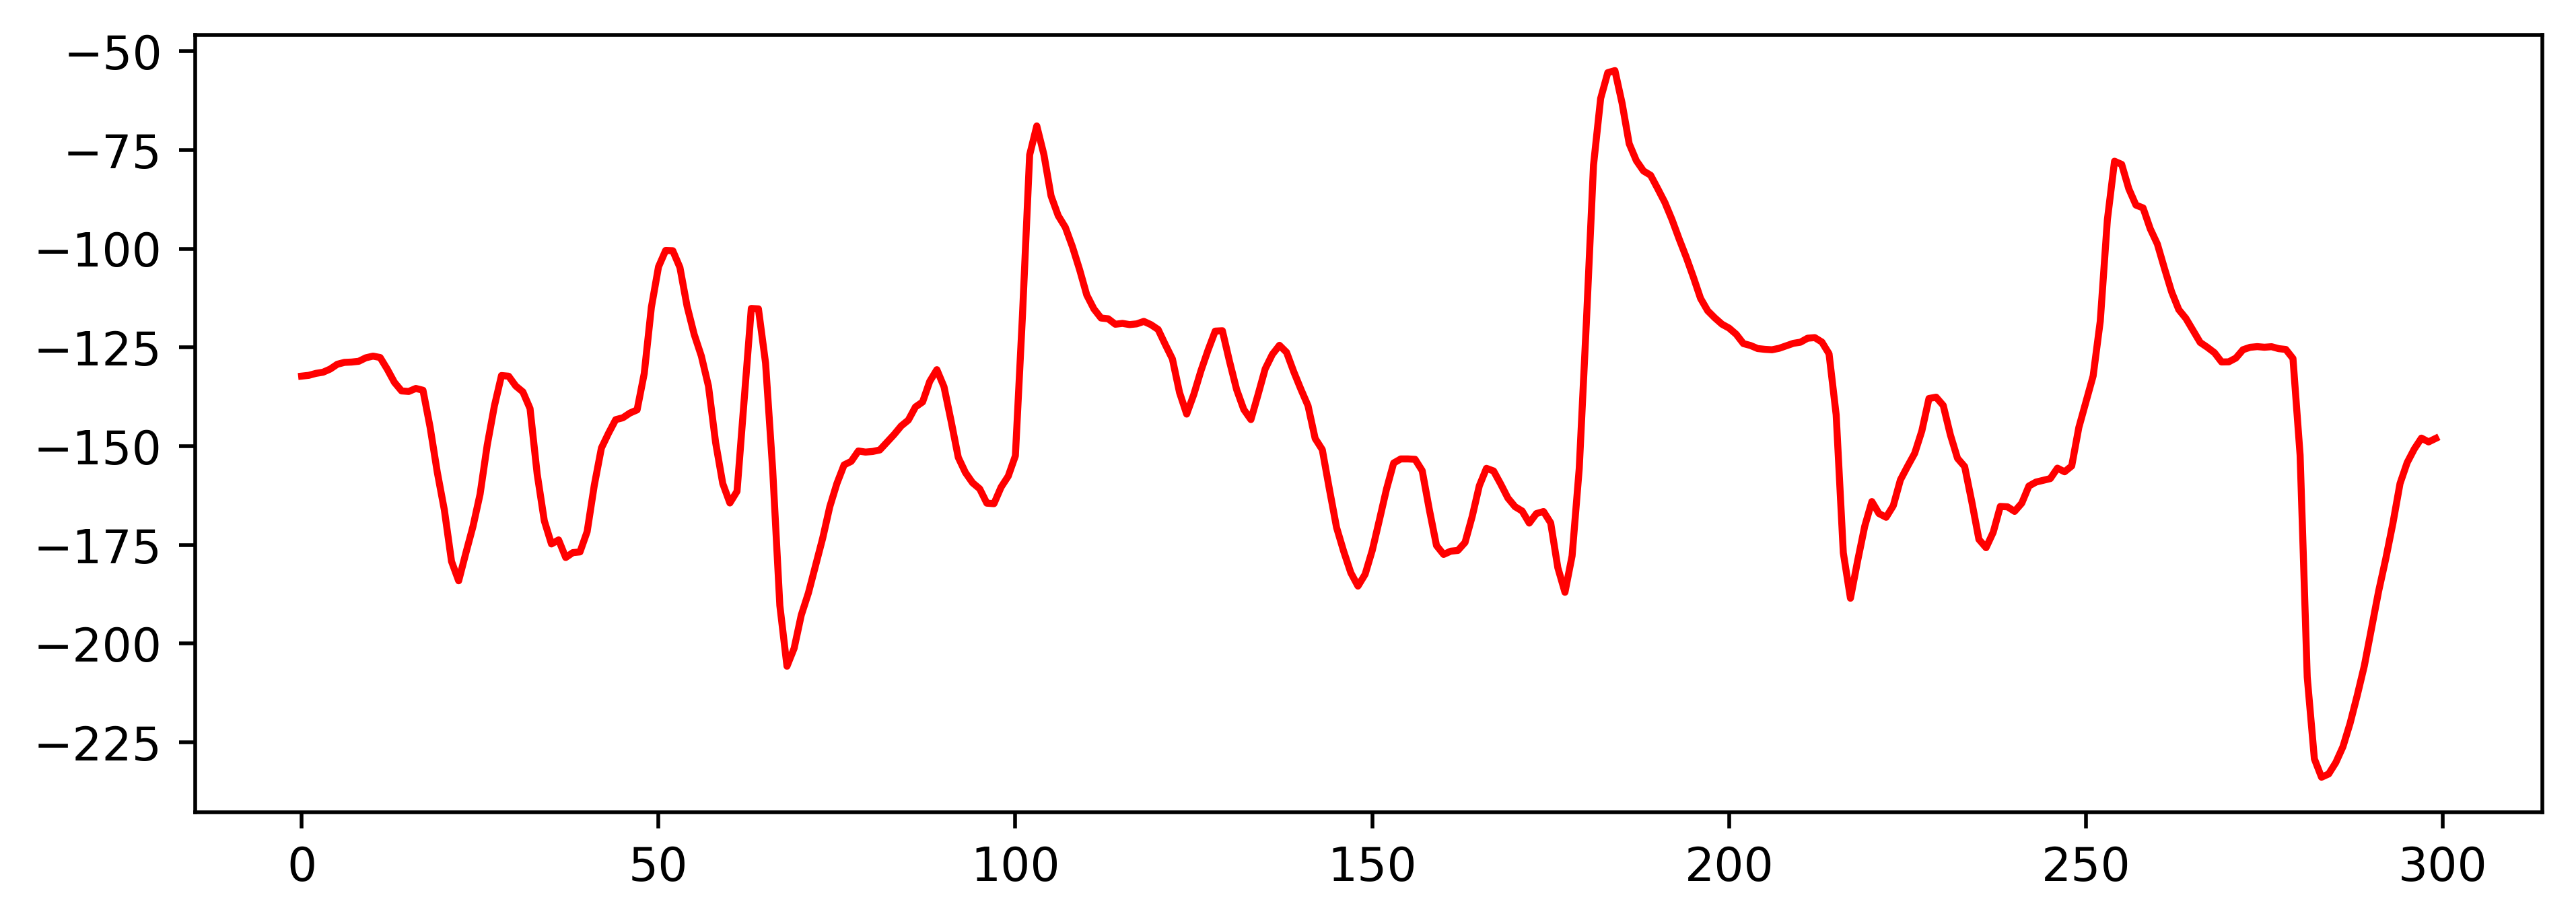
\includegraphics[width=0.45\linewidth]{img/samples/butppg_111004.png} \\
	\end{tabular}
	\caption{Samples of the four signals of the subject with id equal to 11 (where the first subject has id 0). The ``Good'' signals color is blue, while the ``Bad'' signals are red. In those graphs, the vertical dimension is the average of all pixels intensity in a frame, while the horizontal dimension is the time instant in frames. Notice that, since those records are 10 seconds long, it's implied that the sampling frequency is 30 Hz.}
	\label{fig:butppg_samples}
\end{figure}
